\documentclass{article}
\usepackage{amsmath,amssymb,amsthm,booktabs,graphicx}
\usepackage[hidelinks]{hyperref}
\DeclareMathOperator*{\argmax}{arg\,max}
\newtheorem{theorem}{Theorem}[section]
\newtheorem{proposition}[theorem]{Proposition}
\newtheorem{lemma}[theorem]{Lemma}
\newtheorem{corollary}[theorem]{Corollary}
\newtheorem{conjecture}[theorem]{Conjecture}
\newtheorem{openquestion}[theorem]{Open question}
\theoremstyle{definition}
\newtheorem{definition}[theorem]{Definition}
\newtheorem{example}[theorem]{Example}
\theoremstyle{remark}
\newtheorem{remark}[theorem]{Remark}
\newcommand{\Z}{\mathbb{Z}}
\newcommand{\E}{\mathbb{E}}
\newcommand{\Prob}{\mathbb{P}}
\newcommand{\ccrit}{c_{\mathrm{crit}}}

\title{Optimal Additive Integer Masks for One-Guess Vulnerability under an Absolute-Moment Budget}

\author{Joonas P\"a\"akk\"onen\\ Dalarna University, Borl\"ange, Sweden\\ \texttt{jpa@du.se}}

\begin{document}
\maketitle

\begin{abstract}
We study the average one-guess success probability of an adversary who observes the ordinary integer sum of a finite-support secret and an independent integer-valued mask, subject to an absolute-moment budget on the mask. For a uniform secret on an interval the exact optimum and an explicit optimiser are obtained. For a biased bit the masks that achieve no increase over the prior baseline are characterised and their minimal cost is determined. The entire cost--vulnerability frontier is then determined for every bias. It is the piecewise-linear interpolation of an explicit sequence of points generated by cost-optimally shifted truncated geometric masks. It has infinitely many affine pieces, which accumulate at the critical cost, where the frontier meets the prior baseline with zero slope. The proof rests on a layer-cake decomposition of an arbitrary mask into truncated geometrics, along which both the vulnerability and the cost are exactly additive. The results give exact design guidance for additive integer noise under the average one-guess metric; they do not constitute a cryptographic masking scheme.
\end{abstract}

\begin{center}
\textit{Keywords:} Bayes vulnerability, quantitative information flow, additive noise, absolute-moment constraint, geometric distributions.
\end{center}

\section{Introduction}
Quantitative information flow measures how much an observation helps an adversary guess a secret. The most basic operational criterion is the probability that the adversary's single best guess is correct. This is the Bayes vulnerability \(V(X)=\max_x\Prob(X=x)\) before the observation and the posterior vulnerability
\[
V(X\mid S)=\sum_s\max_x\Prob(X=x,S=s)
\]
after observing \(S\)~\cite{Smith09}. The average conditional min-entropy is \(-\log_2 V(X\mid S)\)~\cite{DORS08}. Minimising \(V(X\mid S)\) is therefore equivalent to maximising average conditional min-entropy. Maximal leakage~\cite{IWK20}, worst-case posterior confidence, mutual information, and differential privacy answer different threat models and are not studied here.

We consider the channel \(S=X+Y\) in which an independent integer-valued mask \(Y\) (finite or infinite support) is added to a finite-support integer-valued secret \(X\). The design question is how to choose the law \(q\) of \(Y\) so as to minimise average one-guess success subject to \(\E|Y|\le c\). Absolute-moment costs arise when the practical price of noise is proportional to its magnitude. Zero additional average guessing advantage does not imply independence or perfect secrecy.

\paragraph{Contributions.}
\begin{enumerate}
\item For a uniform secret on an interval of length \(m\) the exact minimal vulnerability and an explicit optimiser are determined (Theorem~\ref{thm:uniform}).
\item For a biased bit all masks that produce no extra average guessing advantage are characterised, the exact critical cost and the strict gap below it are given, and the exact initial segment is determined (Theorems~\ref{thm:zero}--\ref{thm:initial}).
\item For every bias \(p\in(1/2,1)\) the complete frontier is determined (Theorem~\ref{thm:frontier}). It is the linear interpolation of explicit points \(Q_k\), \(k\ge1\), obtained from truncated geometric masks of length \(k\), and it has infinitely many affine pieces accumulating at the critical cost (Corollary~\ref{cor:pieces}). On every piece an optimiser is a mixture of two adjacent truncated geometrics, with a free residual at exactly one endpoint (Corollary~\ref{cor:structure}). The first two pieces beyond the initial segment, which can also be certified directly by dual multipliers, are recovered as special cases (Corollary~\ref{cor:cells}). Figure~\ref{fig:frontier} shows the proved frontier.
\end{enumerate}

\section{Related work}
Smith~\cite{Smith09} introduced Bayes vulnerability and min-entropy leakage. Dodis, Ostrovsky, Reyzin and Smith~\cite{DORS08} defined average min-entropy. Braun, Chatzikokolakis and Palamidessi~\cite{BCP09} compared additive and multiplicative one-try leakage. Issa, Wagner and Kamath~\cite{IWK20} showed that maximal leakage for finite alphabets equals \(\log\sum_s\max_{x:p(x)>0}\Prob(S=s\mid X=x)\).

Saeidian, Cervia, Oechtering and Skoglund~\cite{SCOS21} solved a privacy--utility problem under maximal leakage and expected Hamming distortion; the mechanisms here are restricted to be additive and the cost is an absolute moment. Asoodeh et al.~\cite{Asoodeh17} studied privacy-constrained guessing probabilities under a different formulation that does not specialise to additive integer masks with an absolute-moment budget. Geng, Ding, Guo and Kumar~\cite{GDGK19} derived optimal additive noise for differential privacy under \(\ell_1\) and \(\ell_2\) costs; the constraint is differential privacy, not Bayes vulnerability.

Side-channel masking literature (e.g., the noisy-leakage model of Prouff and Rivain~\cite{PR13}) addresses a different threat model based on shares. A targeted search of the primary quantitative-information-flow, maximal-leakage, differential-privacy-noise, and guessing-with-noise literature did not locate prior solutions of the exact cost-constrained additive-integer problems studied here. This is an observation about the sources examined, not a proof of novelty. The modular analogue \(S=X+Y\bmod n\) is treated in a companion manuscript in preparation~\cite{Pmod}; it is not used here.

\section{Preliminaries}
Let \(X\) have finite support and law \(p\), and let \(Y\) be independent with law \(q\) on \(\Z\). Set \(S=X+Y\).

\begin{proposition}[MAP rule]\label{prop:map}
The optimal one-guess success probability is
\[
V(X\mid S)=\sum_{s\in\Z}\max_x p(x)q(s-x),
\]
attained by any \(g(s)\in\argmax_x p(x)q(s-x)\). In particular \(V(X\mid S)\ge V(X)\).
\end{proposition}
\begin{proof}
A strategy \(g\) succeeds with probability \(\sum_s p(g(s))q(s-g(s))\); maximise each term separately. For any fixed \(x_0\), the sum is at least \(p(x_0)\).
\end{proof}

For a fixed secret distribution the optimisation is over all probability laws \(q\) on \(\Z\) with \(\E_q|Y|\le c\). The optimal value is denoted \(V^*(c)\).

\section{Uniform interval secret}
Let \(X\) be uniform on \(I_m=\{0,\dots,m-1\}\). Then
\[
V(q)=\frac1m\sum_s\max_{x\in I_m}q(s-x).
\]

\begin{lemma}[Layer cake]\label{lem:layer}
Let \(h=\|q\|_\infty\) and \(B_t=\{y:q(y)>t\}\). Then \(mV(q)=\int_0^h|B_t+I_m|\,dt\).
\end{lemma}
\begin{proof}
For each \(s\), \(\max_{y\in s-I_m}q(y)=\int_0^h\mathbf 1[s\in B_t+I_m]\,dt\). Sum over \(s\) and apply Tonelli's theorem.
\end{proof}

\begin{lemma}[One-dimensional sumset]\label{lem:sumset}
For nonempty finite \(A\subset\Z\), \(|A+I_m|\ge|A|+m-1\). For \(m\ge2\), equality holds if and only if \(A\) is an interval of integers.
\end{lemma}
\begin{proof}
\(A+I_m\supseteq A\cup(\max A+I_m)\), and the two sets meet only in \(\max A\). If \(A\) is an interval the sumset is an interval of the stated cardinality. If consecutive elements of \(A\) differ by at least \(2\), a gap point appears in the sumset.
\end{proof}

\begin{lemma}[Cheapest mask of given peak]\label{lem:fill}
For \(h\in(0,1]\) let \(r\ge0\) satisfy \(1/(2r+3)<h\le1/(2r+1)\) and \(\rho=1-(2r+1)h\in[0,2h)\). Let \(q_h\) place mass \(h\) on each of \(\{-r,\dots,r\}\) and \(\rho/2\) on each of \(\pm(r+1)\). Then \(\E_q|Y|\ge C(h):=\E_{q_h}|Y|=(r+1)(1-(r+1)h)\) for every \(q\) with \(\|q\|_\infty\le h\).
\end{lemma}
\begin{proof}
Direct computation gives the cost formula. Let \(R=r+1\) and \(\Delta=q-q_h\). For \(|y|<R\) both factors \(|y|-R\le0\) and \(\Delta(y)\le0\), so their product is nonnegative. For \(|y|=R\) the term vanishes. For \(|y|>R\) both factors are nonnegative. Hence \(\sum(|y|-R)\Delta(y)\ge0\).
\end{proof}

\begin{theorem}[Uniform secret]\label{thm:uniform}
Let \(r\ge0\) satisfy \(r(r+1)/(2r+1)\le c\le(r+1)(r+2)/(2r+3)\). Set \(h^*(c)=(r+1-c)/(r+1)^2\). Then
\[
\min_{\E|Y|\le c}V(q)=\frac{1+(m-1)h^*(c)}{m},
\]
attained by \(q_{h^*(c)}\).
\end{theorem}
\begin{proof}
Lemmas~\ref{lem:layer} and~\ref{lem:sumset} together with \(\int_0^h|B_t|\,dt=1\) give \(mV(q)\ge1+(m-1)\|q\|_\infty\). The cost constraint and Lemma~\ref{lem:fill} force \(\|q\|_\infty\ge h^*(c)\). The candidate has cost exactly \(c\) and interval superlevel sets, so equality holds throughout. The argument covers infinite-support competitors. For \(m=1\) or \(c=0\) one has \(V\equiv1\).
\end{proof}

The optimiser is not in general uniform on an interval. Asymptotically, the cost of a height-\(h\) filled peak is \(C(h)\sim1/(4h)\) (the continuous water-filling limit), so \(h^*(c)\sim1/(4c)\).

\section{Biased bit}
Let \(\Prob(X=0)=p\in(1/2,1)\), \(\Prob(X=1)=1-p\), and \(a=(1-p)/p\in(0,1)\). Define
\[
V_p(q)=\sum_s\max\bigl\{p\,q(s),(1-p)q(s-1)\bigr\}
\]
and
\[
V_p^*(c)=\inf\{V_p(q):\E_q|Y|\le c\}.
\]
The baseline is \(V(X)=p\). Equivalently,
\[
V_p(q)=p+\sum_s\max\bigl(0,(1-p)q(s-1)-p\,q(s)\bigr).
\]
For \(p=1/2\) the problem is the case \(m=2\) of Theorem~\ref{thm:uniform}.

\begin{theorem}[Zero extra average advantage]\label{thm:zero}
\(V_p(q)=p\) if and only if \(q(s)\ge a\,q(s-1)\) for every \(s\in\Z\). Such laws are precisely the mixtures \(q=\sum_L w_L G_L\), where \(G_L(s)=(1-a)a^{s-L}\mathbf{1}_{s\ge L}\), \(w_L\ge0\) and \(\sum_L w_L=1\).
\end{theorem}
\begin{proof}
The first claim is immediate from the excess representation. Given the inequality, set \(d(s)=q(s)-a\,q(s-1)\ge0\). Iterating and using \(a^n q(s-n)\to0\) yields \(q(s)=\sum_{L\le s}d(L)a^{s-L}\). Summing over \(s\) gives \(\sum d(L)=1-a\), so the weights \(w_L=d(L)/(1-a)\) produce the claimed mixture. Conversely each \(G_L\) satisfies the inequality, which is preserved by mixtures.
\end{proof}

\begin{corollary}
No finite-support mask achieves \(V_p(q)=p\). If \(q(s_0)>0\) then the ratio inequality forces \(q(s_0+k)\ge a^k q(s_0)>0\) for all \(k\ge0\).
\end{corollary}

\begin{remark}
\(V_p(q)=p\) concerns the average only. For a pure geometric the posterior at the left endpoint equals \(1\), and \(S\) is never independent of \(X\).
\end{remark}

\begin{theorem}[Critical cost]\label{thm:ccrit}
\[
c_{\mathrm{crit}}(p)=\min_{\ell\in\Z_{\ge0}}\Bigl(\ell+\frac{a(2a^\ell-1)}{1-a}\Bigr),
\]
attained at \(\ell^*=\#\{j\ge1:a^j>1/2\}=\lceil\log2/\log(1/a)\rceil-1\) (an integer median; with a tie when \(a^{\ell^*+1}=1/2\)). Moreover \(V_p^*(c)=p\) for \(c\ge c_{\mathrm{crit}}(p)\) and \(V_p^*(c)>p\) for \(c<c_{\mathrm{crit}}(p)\).
\end{theorem}
\begin{proof}
By Theorem~\ref{thm:zero} and linearity the cost of a zero-advantage mask is at least the minimum over pure shifts. For positive shifts the cost is larger, so it suffices to minimise \(f(\ell)=\E|G-\ell|\) over \(\ell\ge0\). The difference \(f(\ell+1)-f(\ell)=1-2a^{\ell+1}\) changes sign at the stated integer, with a tie exactly when equality holds.

Existence of minimisers: a minimising sequence with \(\E|Y|\le c\) is tight by Markov's inequality. A diagonal argument yields a subsequence converging pointwise to some \(q\). Tightness implies \(\sum q=1\). Fatou's lemma gives \(\E_q|Y|\le c\). Scheff\'e's lemma then upgrades the convergence to \(\ell^1\). The bound \(|V_p(q)-V_p(q')|\le\|q-q'\|_1\) gives continuity of the objective, so a minimiser exists. (The case \(c=0\) is covered by Theorem~\ref{thm:initial}.) If \(V_p^*(c)=p\) for some \(c<c_{\mathrm{crit}}(p)\), the minimiser would be a zero-advantage mask of cost strictly below \(c_{\mathrm{crit}}(p)\), a contradiction. For \(c\ge c_{\mathrm{crit}}(p)\) the geometric at the optimal shift is feasible.
\end{proof}

\begin{theorem}[Initial segment]\label{thm:initial}
For \(0\le c\le1-p\), \(V_p^*(c)=1-pc\), attained by \(q=(1-c)\delta_0+c\delta_1\). Moreover \(V_p(q)\ge1-p\,\E|Y|\) for every \(q\).
\end{theorem}
\begin{proof}
Choosing the first term of the maximum for \(s\le0\) and the second for \(s\ge1\),
\begin{align*}
V_p(q)&\ge p\Pr(Y\le0)+(1-p)\Pr(Y\ge0)\\
&=1-p\Pr(Y>0)-(1-p)\Pr(Y<0)\\
&\ge1-p\Pr(Y\ne0)\ge1-p\,\E|Y|,
\end{align*}
using \(1-p<p\) and \(\mathbf 1[y\ne0]\le|y|\) on \(\Z\). The two-point mask has cost \(c\) and vulnerability \(1-pc\) on the stated interval.
\end{proof}

\subsection{The complete frontier}
\begin{proposition}[Monotonicity and convexity]\label{prop:convex}
The function \(V_p^*\) is nonincreasing and convex on \([0,\infty)\). It is continuous on \((0,\infty)\). Continuity at \(0\) follows from Theorem~\ref{thm:initial}.
\end{proposition}
\begin{proof}
If \(c\le c'\) the feasible set for \(c\) is contained in that for \(c'\), so \(V_p^*\) is nonincreasing. The function \(V_p\) is convex, since a maximum of linear functions is convex and sums of convex functions are convex. For convexity, take feasible masks \(q_0,q_1\) for budgets \(c_0,c_1\) and \(\theta\in[0,1]\). The mixture \(\theta q_0+(1-\theta)q_1\) is feasible for \(\theta c_0+(1-\theta)c_1\) and, by convexity of \(V_p\), has vulnerability at most the corresponding convex combination. Taking infima yields convexity of \(V_p^*\). A finite convex function on an open interval is continuous, so \(V_p^*\) is continuous on \((0,\infty)\).
\end{proof}

\begin{definition}[Truncated geometrics and the points \(Q_k\)]\label{def:Q}
For \(L\in\Z\) and \(k\in\{1,2,\dots\}\) let
\[
T_{L,k}(s)=\frac{1-a}{1-a^k}\,a^{s-L}\,\mathbf 1\{L\le s\le L+k-1\},
\]
and put \(T_{L,\infty}=G_L\). For \(k\ge1\) and \(m\ge0\) write
\[
u_k=\frac{a^k}{1-a^k},\qquad A_m=\sum_{i=1}^m a^i=\frac{a(1-a^m)}{1-a},
\]
\[
m_k=\#\{1\le j\le k-1:\ 2a^j>1+a^k\},
\]
and define
\[
V_k=p+(2p-1)\,u_k,\qquad C_k=\frac{a}{1-a}+(m_k-2A_{m_k})+u_k\bigl(2(m_k-A_{m_k})-k\bigr),
\]
\(Q_k=(C_k,V_k)\), and \(Q_\infty=(\ccrit(p),p)\). An index \(k\) is a \emph{transition} if \(m_{k+1}=m_k+1\), and a \emph{tie} if \(2a^{m_k+1}=1+a^k\).
\end{definition}

For example \(Q_1=(0,1)\) is the point mass \(\delta_0\) and \(Q_2=(1-p,\,1-p+p^2)\).

\begin{theorem}[Complete biased-bit frontier]\label{thm:frontier}
Let \(p\in(1/2,1)\). Then \(0=C_1<C_2<C_3<\cdots\), \(C_k\to\ccrit(p)\), \(V_k\downarrow p\), and
\[
V_p^*(c)=\begin{cases}
V_k-\sigma_k\,(c-C_k), & C_k\le c\le C_{k+1},\ k\ge1,\\
p, & c\ge\ccrit(p),
\end{cases}
\]
with slopes
\[
\sigma_k=\frac{V_k-V_{k+1}}{C_{k+1}-C_k}=\frac{2p-1}{E_k},\qquad E_k=k-A_k-2(m_k-A_{m_k})-\theta_k(1-a^k),
\]
where
\[
\theta_k=\begin{cases}0,& m_{k+1}=m_k,\\[1mm] \dfrac{2a^{m_k+1}-1-a^{k+1}}{a^k(1-a)}\in(0,1],& m_{k+1}=m_k+1.\end{cases}
\]
The slopes satisfy \(\sigma_1\ge\sigma_2\ge\cdots>0\) and \(\sigma_k\to0\), and \(\sigma_{k-1}=\sigma_k\) holds if and only if \(k\) is a tie. For \(C_k\le c\le C_{k+1}\) an optimiser is
\[
q_c=\vartheta\,T_{-m_k,k}+(1-\vartheta)\,T_{-m_{k+1},k+1},\qquad \vartheta=\frac{C_{k+1}-c}{C_{k+1}-C_k},
\]
and for \(c\ge\ccrit(p)\) an optimiser is \(G_{-\ell^*}\).
\end{theorem}

Equivalently, \(V_p^*\) is the lower convex envelope of \(\{Q_k:k\ge1\}\cup\{Q_\infty\}\), extended by the constant \(p\), and every \(Q_k\) lies on the frontier.

\begin{corollary}[Infinitely many pieces]\label{cor:pieces}
For every \(p\in(1/2,1)\) the frontier has infinitely many affine pieces on \([0,\ccrit(p))\), and they accumulate only at \(\ccrit(p)\). The left derivative of \(V_p^*\) at \(\ccrit(p)\) is \(0\), so \(V_p^*\) is differentiable there. The set of biases with at least one tie is
\[
\mathcal T=\{p\in(1/2,1):\ 2a^j=1+a^k\ \text{for some integers }1\le j<k\}.
\]
It is countable and contains \(\varphi:=(\sqrt5-1)/2\) (take \(j=1,k=3\)). If \(p\notin\mathcal T\), the intervals \([C_k,C_{k+1}]\) are exactly the maximal affine pieces of \(V_p^*\) on \([0,\ccrit(p)]\). If \(p\in\mathcal T\), at most \(\ell^*\) adjacent pairs merge.
\end{corollary}

\begin{corollary}[Structure of the optimisers]\label{cor:structure}
Suppose first that \(m_{k+1}=m_k=m\). Then on \([C_k,C_{k+1}]\) the optimiser \(q_c\) is supported on \(\{-m,\dots,k-m\}\). It has ratio exactly \(a\) on \(\{-m,\dots,k-m-1\}\) and a free residual at the right endpoint. Suppose instead that \(m_{k+1}=m_k+1=m+1\). Then \(q_c\) is supported on \(\{-m-1,\dots,k-m-1\}\). It has ratio exactly \(a\) on \(\{-m,\dots,k-m-1\}\) and a free residual at the left endpoint. Thus every piece has an optimiser that is residual-adjusted, with a free residual at exactly one endpoint.
\end{corollary}

\subsection{Proof of the complete frontier}
\begin{lemma}[Geometric layer cake]\label{lem:geolayer}
Let \(q\) be a probability law on \(\Z\) with \(\E_q|Y|<\infty\). There is a probability measure \(\nu\) on pairs \((L,k)\in\Z\times\{1,2,\dots,\infty\}\) such that
\[
q=\int T_{L,k}\,d\nu,\qquad V_p(q)=\int V_p(T_{L,k})\,d\nu,\qquad \E_q|Y|=\int \E_{T_{L,k}}|Y|\,d\nu .
\]
\end{lemma}
\begin{proof}
Put \(w(s)=q(s)a^{-s}\ge0\). Since \(q\le1\), \(w(s)\to0\) as \(s\to-\infty\). Hence for \(t>0\) the level set \(\{w>t\}\) is bounded below, and it is a disjoint union of maximal integer intervals (components) \(I=[L,L+k-1]\), \(k\in\{1,\dots,\infty\}\). For a component \(I\) write \(g_I(s)=a^s\mathbf 1_I(s)\). Its mass is \(M_I=a^L(1-a^k)/(1-a)\), and \(g_I=M_I\,T_{L,k}\). By the layer-cake formula and Tonelli's theorem,
\[
q(s)=a^s\int_0^\infty\mathbf 1\{w(s)>t\}\,dt=\int_0^\infty\sum_{I}g_I(s)\,dt ,
\]
where the sum runs over the components of \(\{w>t\}\). Let \(\nu\) be the image of \(dt\otimes\sum_I M_I\delta_I\) under \(I=[L,L+k-1]\mapsto(L,k)\). Its total mass is \(\sum_s q(s)=1\). The first identity is the display, and the cost identity follows from it by Tonelli's theorem.

For the vulnerability, use the excess representation. Since \(a\,q(s-1)-q(s)=a^s\bigl(w(s-1)-w(s)\bigr)\),
\[
\bigl(w(s-1)-w(s)\bigr)_+=\int_0^\infty\mathbf 1\{w(s-1)>t\ge w(s)\}\,dt .
\]
The integrand is \(1\) exactly when \(s-1\) is the right end of a finite component of \(\{w>t\}\). Hence
\[
\sum_s\bigl(a\,q(s-1)-q(s)\bigr)_+=\int_0^\infty\sum_{I\ \text{finite}}a^{L+k}\,dt .
\]
For a finite component the same quantity computed for \(g_I\) alone is \(a^{L+k}\), from its single down-step at \(s=L+k\). For an infinite component it is \(0\). The map \(g\mapsto p\sum g+p\sum_s(a\,g(s-1)-g(s))_+\) is positively homogeneous and extends \(V_p\). Therefore \(V_p(q)=\int V_p(T_{L,k})\,d\nu\).
\end{proof}

The point of Lemma~\ref{lem:geolayer} is that \(V_p\), which is only convex in general, is exactly linear along this decomposition. It plays the role for the biased bit that Lemma~\ref{lem:layer} plays for the uniform secret.

\begin{lemma}[Truncated geometrics]\label{lem:T}
\begin{enumerate}
\item \(V_p(T_{L,k})=V_k\) for all \(L\in\Z\) and \(k\ge1\), and \(V_p(G_L)=p\).
\item \(\min_{L\in\Z}\E_{T_{L,k}}|Y|=C_k\), attained at \(L=-m_k\).
\item \(m_k\) is nondecreasing in \(k\), and \(m_{k+1}-m_k\in\{0,1\}\). No two consecutive indices are transitions. Moreover \(m_2=0\), and \(m_k=\ell^*\) for all large \(k\).
\end{enumerate}
\end{lemma}
\begin{proof}
(1) By the proof of Lemma~\ref{lem:geolayer}, \(V_p(T_{L,k})=p+p\,a^{L+k}/M_I=p+p(1-a)u_k\), and \(p(1-a)=2p-1\). The second claim is Theorem~\ref{thm:zero}.

(2) For \(L\ge0\) all atoms are nonnegative, so the cost increases with \(L\). For \(L\le-k\) all atoms are negative, so it decreases with \(L\). For \(L=-m\) with \(0\le m\le k-1\), let \(J=Y+m\), a truncated geometric on \(\{0,\dots,k-1\}\). Then \(\E|Y|=\E J-m+2\E(m-J)_+\). Here \(\E J=a/(1-a)-k\,u_k\) and \(\E(m-J)_+=(m-A_m)(1+u_k)\). Hence
\[
C_k(m):=\E_{T_{-m,k}}|Y|=\frac{a}{1-a}+(m-2A_m)+u_k\bigl(2(m-A_m)-k\bigr)\qquad(0\le m\le k).
\]
Using \(A_{m+1}-A_m=a^{m+1}\),
\begin{equation}\label{eq:shift}
C_k(m+1)-C_k(m)=\frac{1+a^k-2a^{m+1}}{1-a^k}.
\end{equation}
This difference is increasing in \(m\), and it is negative exactly when \(2a^{m+1}>1+a^k\). Since \(2a^j\) decreases in \(j\), the minimiser is \(m=m_k\).

(3) Monotonicity holds because \(1+a^k\) decreases in \(k\). Suppose \(m\) increased by \(2\) in one step, or there were transitions at both \(k\) and \(k+1\). Either case requires \(2a^{m+2}>1+a^{k+2}\) and \(2a^{m+1}\le1+a^{k}\) for some \(m\). Then \(1+a^{k+2}<a(1+a^k)\), that is, \(1-a<a^{k+1}(1-a)\), which is impossible. \(m_2=0\) because \(2a>1+a^2\) never holds. As \(k\to\infty\), \(m_k\to\#\{j\ge1:2a^j>1\}=\ell^*\).
\end{proof}

\begin{lemma}[Convex position]\label{lem:convexpos}
Let \(E_k=(C_{k+1}-C_k)/(u_k-u_{k+1})\). Then \(E_k\) is given by the formula of Theorem~\ref{thm:frontier}, and \(E_1=1-a\). For \(k\ge2\) the increment \(E_k-E_{k-1}\) equals
\begin{itemize}
\item \(1-a^k\) if neither \(k-1\) nor \(k\) is a transition;
\item \((1-\theta_k)(1-a^k)\) if \(k\) is a transition;
\item \(\bigl(2a^{m_k}-1-a^{k}\bigr)+\theta_{k-1}(1-a^{k-1})\) if \(k-1\) is a transition.
\end{itemize}
In particular \(E_k\) is nondecreasing, \(E_k\ge1-a>0\), and \(E_k\to\infty\). Moreover \(E_k=E_{k-1}\) if and only if \(k\) is a tie.
\end{lemma}
\begin{proof}
Note that \(u_k-u_{k+1}=a^k(1-a)/\bigl((1-a^k)(1-a^{k+1})\bigr)>0\) and \(k u_k-(k+1)u_{k+1}=(u_k-u_{k+1})(k-A_k)\). If \(m_{k+1}=m_k=m\), the formula for \(C_k(m)\) gives \(E_k=k-A_k-2(m-A_m)\). If \(k\) is a transition, then \(C_{k+1}=C_{k+1}(m+1)=C_{k+1}(m)-\delta\) by~\eqref{eq:shift}, with \(\delta=(2a^{m+1}-1-a^{k+1})/(1-a^{k+1})\). Dividing, \(\delta/(u_k-u_{k+1})=\theta_k(1-a^k)\). The condition \(m_{k+1}=m+1\) gives \(2a^{m+1}>1+a^{k+1}\), and \(m_k=m\) gives \(2a^{m+1}\le1+a^k\). Together, \(0<2a^{m+1}-1-a^{k+1}\le a^k(1-a)\), so \(\theta_k\in(0,1]\), with \(\theta_k=1\) exactly at a tie. Conversely, a tie forces a transition, since \(1+a^k>1+a^{k+1}\).

The three differences follow from \(A_k-A_{k-1}=a^k\) and \(2\bigl((m+1)-A_{m+1}\bigr)-2(m-A_m)=2(1-a^{m+1})\). By Lemma~\ref{lem:T}(3) the three cases are exhaustive. In the third case \(2a^{m_k}-1-a^k>0\) is the transition condition at \(k-1\). Finally, \(E_1=1-A_1=1-a\) because \(m_1=m_2=0\), and \(E_k\ge k-A_k-2\ell^*-1\to\infty\).
\end{proof}

\begin{lemma}\label{lem:limit}
\(C_k\to\ccrit(p)\) and \(V_k\to p\).
\end{lemma}
\begin{proof}
\(V_k\to p\) is clear. For every \(L\) and \(k\), \(G_L=(1-a^k)T_{L,k}+a^kG_{L+k}\). Taking \(L=-\ell^*\) gives \(C_k\le\E_{T_{-\ell^*,k}}|Y|\le\ccrit(p)/(1-a^k)\). Taking \(L=-m_k\) and using Theorem~\ref{thm:ccrit} gives \(\ccrit(p)\le(1-a^k)C_k+a^k\bigl(k+a/(1-a)\bigr)\). Both bounds tend to \(\ccrit(p)\).
\end{proof}

\begin{proof}[Proof of Theorem~\ref{thm:frontier}]
Let \(g\) be the right-hand side of the theorem, with \(\sigma_k=(V_k-V_{k+1})/(C_{k+1}-C_k)\). Since \(V_k-V_{k+1}=(2p-1)(u_k-u_{k+1})\), we have \(\sigma_k=(2p-1)/E_k\). By Lemma~\ref{lem:convexpos}, \(C_k\) is strictly increasing, and \(\sigma_k\) is positive, nonincreasing and tends to \(0\). With Lemma~\ref{lem:limit}, \(g\) is well defined, continuous, nonincreasing and convex on \([0,\infty)\), since its slopes \(-\sigma_1\le-\sigma_2\le\dots\le0\) are nondecreasing. Also \(g(C_k)=V_k\) and \(g(\ccrit)=p\).

\emph{Lower bound.} Let \(\E_q|Y|\le c\), and let \(\nu\) be as in Lemma~\ref{lem:geolayer}. Set \(C_\infty=\ccrit(p)\) and \(V_\infty=p\). By Lemma~\ref{lem:T} and Theorem~\ref{thm:ccrit}, \(V_p(T_{L,k})=V_k\) and \(\E_{T_{L,k}}|Y|\ge C_k\) for all \(k\le\infty\). We use \(g(C_k)=V_k\), then Jensen's inequality for the convex function \(g\) (all \(C_k\) lie in \([0,\ccrit]\)), then monotonicity of \(g\):
\[
V_p(q)=\int V_k\,d\nu=\int g(C_k)\,d\nu\ \ge\ g\Bigl(\int C_k\,d\nu\Bigr)\ \ge\ g\bigl(\E_q|Y|\bigr)\ \ge\ g(c).
\]

\emph{Upper bound.} For \(C_k\le c\le C_{k+1}\), Lemma~\ref{lem:T}(2) shows that \(q_c\) has cost \(\vartheta C_k+(1-\vartheta)C_{k+1}=c\). By convexity of \(V_p\) and Lemma~\ref{lem:T}(1), \(V_p(q_c)\le\vartheta V_k+(1-\vartheta)V_{k+1}=g(c)\). For \(c\ge\ccrit(p)\), \(G_{-\ell^*}\) is feasible and has \(V_p=p\). Hence \(V_p^*=g\). The statements about the slopes are Lemma~\ref{lem:convexpos}.
\end{proof}

\begin{proof}[Proof of Corollary~\ref{cor:pieces}]
By Lemma~\ref{lem:limit} the pieces \([C_k,C_{k+1}]\) are infinitely many and accumulate only at \(\ccrit\). The left derivative at \(\ccrit\) is \(\lim_k(-\sigma_k)=0\), and the right derivative is \(0\). Two adjacent pieces have equal slopes if and only if \(E_{k-1}=E_k\), that is, if and only if \(k\) is a tie. Suppose \(2a^j=1+a^k\) with \(1\le j<k\). Then exactly \(j-1\) indices \(i\ge1\) satisfy \(2a^i>1+a^k\), so \(j=m_k+1\) and \(k\) is a tie. The converse is the definition. Every tie is a transition, and \(m_k\) increases from \(0\) to \(\ell^*\) in unit steps, so there are at most \(\ell^*\) ties. For \(p=\varphi\) one has \(a=\varphi\), and \(1+\varphi^3=2\varphi\) because \(\varphi^2=1-\varphi\). For fixed \((j,k)\) the equation \(2a^j=1+a^k\) has finitely many roots, so \(\mathcal T\) is countable.
\end{proof}

\begin{proof}[Proof of Corollary~\ref{cor:structure}]
Suppose \(m_{k+1}=m_k=m\). Both components start at \(-m\). On \(\{-m,\dots,k-m-1\}\) the mixture is a positive multiple of \(a^s\), and the atom at \(k-m\) comes only from \(T_{-m,k+1}\). Now suppose \(m_{k+1}=m+1\). The atom at \(-m-1\) comes only from \(T_{-m-1,k+1}\), and on \(\{-m,\dots,k-m-1\}\) both components are multiples of \(a^s\).
\end{proof}

\subsection{The first pieces and explicit dual certificates}
The first pieces of Theorem~\ref{thm:frontier} can also be certified directly. All such certificates use the following weak-duality device. For any \(\alpha:\Z\to[0,1]\),
\begin{equation}\label{eq:weak}
V_p(q)\ge\sum_y\kappa_\alpha(y)q(y),\qquad\kappa_\alpha(y):=p\alpha_y+(1-p)(1-\alpha_{y+1}).
\end{equation}
If \(\kappa_\alpha(y)\ge\mu-\lambda|y|\) for all \(y\) with \(\lambda\ge0\), then \(V_p(q)\ge\mu-\lambda\E_q|Y|\ge\mu-\lambda c\) for every feasible \(q\).

\begin{corollary}[Certified cells]\label{cor:cells}
Let \(1/2<p\le\varphi\), \(a=(1-p)/p\), and
\[
c_1=\frac{1+a^2}{1+a+a^2},\qquad c_2=\frac{1+a^2+2a^3}{1+a+a^2+a^3}.
\]
Then \(1-p<c_1<c_2\) and
\[
V_p^*(c)=\begin{cases}
p+\dfrac{(1-p)^2}{p}(1-c), & 1-p\le c\le c_1,\\[2mm]
1-p+p^3(2-c), & c_1\le c\le c_2.
\end{cases}
\]
On the first piece the optimiser is \(q(-1)=c-a(1-c)\), \(q(0)=1-c\), \(q(1)=a(1-c)\). On the second piece, with \(t=p^2(2-c)\), the optimiser is \(q(-1)=t\), \(q(0)=at\), \(q(1)=a^2t\), \(q(2)=1-t(1+a+a^2)\). Both affine functions are lower bounds on \(V_p^*(c)\) for every \(c\ge0\).
\end{corollary}
\begin{proof}
\emph{Via Theorem~\ref{thm:frontier}.} Since \(2a^j>1+a^k\) never holds for \(2\le j<k\le4\), one has \(m_3=\mathbf 1\{2a>1+a^3\}\) and \(m_4=\mathbf 1\{2a>1+a^4\}\). Now \(1+a^3-2a=(a-1)(a^2+a-1)\) is negative if and only if \(a>\varphi\), that is, \(p<\varphi\). Also \(1+a^4-2a=(a-1)(a^3+a^2+a-1)\) is negative for \(a\ge\varphi\). So for \(p<\varphi\), \(m_3=m_4=1\), and substitution gives \(C_3=c_1\), \(C_4=c_2\), \(\sigma_2=(1-p)^2/p\) and \(\sigma_3=p^3\). The optimisers are \(q_c\) of Theorem~\ref{thm:frontier}. At \(p=\varphi\) the index \(3\) is a tie and both formulas describe a single affine piece. The ordering \(1-p<c_1<c_2\) follows by direct comparison of the rational expressions.

\emph{Independent certificates.} These pieces can also be certified directly by dual multipliers; the certificates are short and checkable by hand.

\emph{First piece, lower bound.} Take \(\alpha_y=1\) for \(y\le0\), \(\alpha_1=(2p-1)/p\), \(\alpha_y=0\) for \(y\ge2\), \(\lambda=(1-p)^2/p\), and \(\mu=p+\lambda\). Then \(\kappa(y)=p\) for \(y\le-1\), \(\kappa(0)=\mu\), \(\kappa(1)=\mu-\lambda\), and \(\kappa(y)=1-p\) for \(y\ge2\). The dual inequality holds with equality at \(y=-1,0,1\) and holds for \(y\le-2\). It holds for \(y\ge2\) if and only if \((1-p)^2\ge p(2p-1)\), i.e., \(p\le\varphi\). Thus \(V_p^*(c)\ge p+\lambda(1-c)\) for all \(c\).

\emph{First piece, attainment.} The displayed mask has mass \(1\) and cost \(c\), and it is nonnegative precisely when \(c\ge1-p\). The ratio constraint \(q(0)\ge a\,q(-1)\) holds precisely when \(c\le c_1\). Direct evaluation of the four nonzero terms of \(V_p\) (\(s=-1,0,1,2\)) yields the claimed value.

\emph{Second piece, lower bound.} Take \(\alpha_y=1\) for \(y\le-1\), \(\alpha_0=p(1+p)\), \(\alpha_1=p^2\), \(\alpha_y=0\) for \(y\ge2\), \(\lambda=p^3\), and \(\mu=1-p+2p^3\). The condition \(p\le\varphi\) ensures all weights lie in \([0,1]\). Direct expansion shows equality of the dual inequality at \(y=-1,0,1,2\), and the inequality holds for \(y\le-2\) and for \(y\ge3\). Thus \(V_p^*(c)\ge1-p+p^3(2-c)\) for all \(c\).

\emph{Second piece, attainment.} The displayed mask has mass \(1\) and cost \(c\). Nonnegativity of the residual holds precisely when \(c\ge c_1\). The residual does not exceed the geometric continuation precisely when \(c\le c_2\). Evaluation of \(V_p\) on the four atoms yields the claimed value.
\end{proof}

\begin{example}
For \(p=3/5\): \(a=2/3\), \(\ell^*=1\), \(\ccrit=5/3\), and \(m_k=1\) for all \(k\ge3\). The vertices begin \(Q_1=(0,1)\), \(Q_2=(2/5,19/25)\), \(Q_3=(13/19,13/19)\), \(Q_4=(11/13,211/325)\), \(Q_5=(213/211,133/211)\). On \([2/5,13/19]\), \(V_p^*(c)=13/15-4c/15\). At \(c=1/2\) the optimiser is \((1/6,1/2,1/3)\) on \(\{-1,0,1\}\) and \(V_p^*=11/15\). At \(c=3/4\) one has \(V_p^*=67/100\), and at \(c=4/5\) one has \(V_p^*=412/625\). At \(c=1\), which lies in \([C_4,C_5]\), the optimiser is \((27,18,12,8,5)/70\) on \(\{-1,\dots,3\}\): geometric with ratio \(2/3\) plus a right residual. Its value is \(V_p^*(1)=221/350\).
\end{example}

\begin{remark}[Biases above \(\varphi\)]
The bias restriction in Corollary~\ref{cor:cells} is genuine. For \(p>\varphi\) one has \(m_3=0\), and the piece after \(1-p\) is \([1-p,C_3]\) with \(C_3=a(1+2a)/(1+a+a^2)\); the first formula of Corollary~\ref{cor:cells} is then not the frontier. At \(p=3/4\) and \(c=3/10\) that formula equals \(97/120\). The mask \(q(0)=51/70\), \(q(1)=17/70\), \(q(2)=2/70\) has cost \(3/10\) and vulnerability \(223/280<97/120\). By Theorem~\ref{thm:frontier} it is optimal: \(c=3/10\) lies in \([C_2,C_3]=[1/4,5/13]\), and \(V_{3/4}^*(3/10)=223/280\).
\end{remark}

\begin{remark}[Optimal ratios need not all equal \(a\)]
At \(p=3/5\) and \(c=1/2\) the optimal mask on \(\{-1,0,1\}\) is \((1/6,1/2,1/3)\). Here \(a=2/3\), but \(q(0)/q(-1)=3\neq a\). Thus an optimal intermediate mask need not have geometric ratios on its entire support. Corollary~\ref{cor:structure} shows that this deviation is confined to a single free residual at one endpoint (here the left one, since \(m_3=m_2+1\)).
\end{remark}

\begin{remark}[Numerical cross-check]
Theorem~\ref{thm:frontier} was cross-checked independently on 336 points between the end of the previously certified pieces and \(\ccrit(p)\), for 14 biases between \(0.52\) and \(0.95\). At each point, floating-point linear programs were turned into rigorous bounds by rounding to rationals and checking feasibility exactly: an upper bound from a finite-window primal mask, and a lower bound from a dual certificate~\eqref{eq:weak} with its tails checked exactly. The two bounds agree with the closed form to within \(3\cdot10^{-11}\), the rounding floor of the certificates. The algebraic ingredients (closed forms of \(C_k\) and \(V_k\), monotonicity of \(E_k\), and Lemma~\ref{lem:geolayer} on random rational masks) were also checked in exact arithmetic. Verification scripts are maintained in the repository \url{https://github.com/fv2fm2z7rk-droid/additive-integer-masks-qif}. None of the proofs depends on these computations.
\end{remark}

Figure~\ref{fig:frontier} displays the cost--vulnerability frontier of Theorem~\ref{thm:frontier} for several biases. All curves are proved.

\begin{figure}[htbp]
\centering
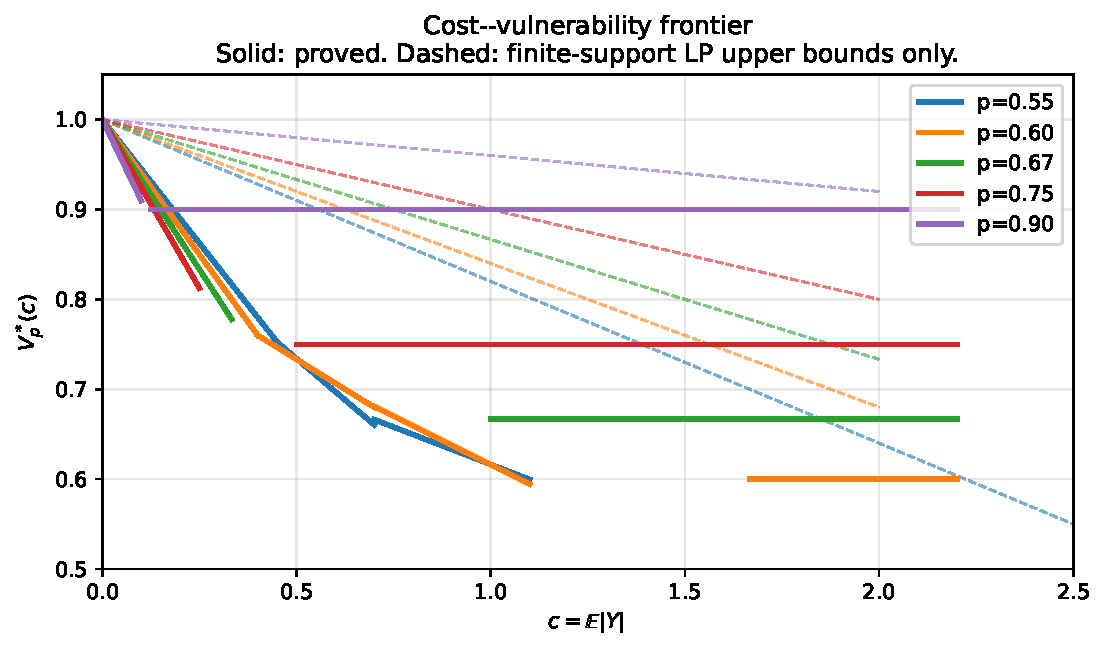
\includegraphics[width=0.85\textwidth]{frontier.pdf}
\caption{Cost--vulnerability frontier \(V_p^*\) from Theorem~\ref{thm:frontier}, computed in exact rational arithmetic. Dots mark the vertices \(Q_k\) (shown while \(V_k-p>10^{-4}\)); bars mark \(\ccrit(p)\). All curves are proved.}
\label{fig:frontier}
\end{figure}

\begin{table}[t]
\centering
\caption{Exact values of \(V_p^*(c)\), from Theorems~\ref{thm:uniform}, \ref{thm:ccrit}, \ref{thm:initial} and~\ref{thm:frontier}. All entries are proved.}
\label{tab:values}
\small
\setlength{\tabcolsep}{4pt}
\begin{tabular}{@{}lcccccc@{}}
\toprule
\(c\) & \(0\) & \(0.25\) & \(0.5\) & \(0.75\) & \(1\) & \(1.5\)\\
\midrule
\(p=1/2\) (uniform \(m=2\)) & \(1\) & \(7/8\) & \(3/4\) & \(21/32\) & \(5/8\) & \(7/12\)\\
\(p=0.6\) & \(1\) & \(17/20\) & \(11/15\) & \(67/100\) & \(221/350\) & \(\frac{758611}{1256830}\)\\
\(p=2/3\) & \(1\) & \(5/6\) & \(11/15\) & \(101/147\) & \(2/3\) & \(2/3\)\\
\(p=3/4\) & \(1\) & \(13/16\) & \(3/4\) & \(3/4\) & \(3/4\) & \(3/4\)\\
\(p=0.9\) & \(1\) & \(0.9\) & \(0.9\) & \(0.9\) & \(0.9\) & \(0.9\)\\
\bottomrule
\end{tabular}
\end{table}

\section{Limitations and future work}
The model is elementary: one observation, one guess, independence, and a pure absolute-moment cost. For the biased bit the frontier is now complete. Three questions remain open. First, uniqueness: Theorem~\ref{thm:frontier} exhibits one optimiser per budget, and whether it is unique (apart from the degeneracy at ties) is not proved. Second, priors on three or more points beyond the uniform case: the proof uses the single likelihood ratio \(a\) of a bit, and no analogous exact linearisation is known for general priors. Third, other cost functions. Extensions to modular arithmetic are treated in a companion manuscript in preparation~\cite{Pmod}; multiple guesses remain open.

\section{Conclusion}
The optimal additive integer masks have been determined for a uniform interval secret and, for a biased bit, along the entire cost--vulnerability frontier: the zero-advantage regime and the critical cost, and below it an explicit piecewise-linear frontier with infinitely many pieces and explicit optimisers. The results supply exact design guidance for the average one-guess metric inside a transparent model. They do not by themselves yield a concrete cryptographic masking scheme, and zero average guessing advantage is not perfect secrecy.

\section*{Acknowledgment}
Portions of the drafting, proof structuring, figure generation, verification scripts, and release packaging were assisted by AI tools (Grok and Grok Bot). The author remains fully responsible for the accuracy of all statements, proofs, and numerical results.

\begin{thebibliography}{10}
\bibitem{Smith09} G.~Smith, ``On the foundations of quantitative information flow,'' in \emph{FoSSaCS 2009}, LNCS 5504. Springer, 2009.
\bibitem{DORS08} Y.~Dodis, R.~Ostrovsky, L.~Reyzin, and A.~Smith, ``Fuzzy extractors: How to generate strong keys from biometrics and other noisy data,'' \emph{SIAM J.\ Comput.}, vol.~38, no.~1, pp.~97--139, 2008.
\bibitem{BCP09} C.~Braun, K.~Chatzikokolakis, and C.~Palamidessi, ``Quantitative notions of leakage for one-try attacks,'' \emph{ENTCS}, vol.~249, pp.~75--91, 2009.
\bibitem{IWK20} I.~Issa, A.~B.~Wagner, and S.~Kamath, ``An operational approach to information leakage,'' \emph{IEEE Trans.\ Inf.\ Theory}, vol.~66, no.~3, pp.~1625--1657, 2020.
\bibitem{SCOS21} S.~Saeidian, G.~Cervia, T.~J.~Oechtering, and M.~Skoglund, ``Optimal maximal leakage-distortion tradeoff,'' in \emph{2021 IEEE Information Theory Workshop (ITW)}, 2021. Full version: arXiv:2105.01033.
\bibitem{Asoodeh17} S.~Asoodeh, M.~Diaz, F.~Alajaji, and T.~Linder, ``Estimation efficiency under privacy constraints,'' \emph{IEEE Trans.\ Inf.\ Theory}, vol.~65, no.~3, pp.~1512--1534, 2019.
\bibitem{PR13} E.~Prouff and M.~Rivain, ``Masking against side-channel attacks: A formal security proof,'' in \emph{EUROCRYPT 2013}, LNCS 7881. Springer, 2013.
\bibitem{GDGK19} Q.~Geng, W.~Ding, R.~Guo, and S.~Kumar, ``Optimal noise-adding mechanism in additive differential privacy,'' in \emph{AISTATS 2019}, 2019. arXiv:1809.10224.
\bibitem{Pmod} J.~P\"a\"akk\"onen, ``Optimal additive modular masks for one-guess vulnerability under a circular-moment budget,'' companion manuscript in preparation, 2026.
\end{thebibliography}
\end{document}
